\subsection{Анализ оптимального расположения маячков в помещении}

Мы имеем начальную систему уравнений, основанную на методе трилатерации:
\[
\begin{cases}
    (x_0-x_1)^2+(y_0-y_1)^2=r_1^2 \\
    (x_0-x_2)^2+(y_0-y_2)^2=r_2^2 \\
    (x_0-x_3)^2+(y_0-y_3)^2=r_3^2 \\
\end{cases}
\]

Однако данная система не может дать однозначного решения в виде точки, если, например, общая область пересечения кругов не является точкой. Назовем в таком случае область такого общего пересечения областью ошибки локализации. Введем также обозначение: пусть величина ошибки варьируется в интервале $(-\epsilon, \epsilon)$. Используя это, определим:
\[
C_{p_i}=
    \{ 
        (x; y) \in R^2 | (x-x_i)^2+(y-y_i)^2 \leq (r_i+\epsilon_i)^2, \\
                                             (x-x_i)^2+(y-y_i)^2 \geq (r_i-\epsilon_i)^2 
    \}
\]

В приведенном выше определении можно заметить, что $\epsilon_i=0, \cap_i C_{p_i}$ образует единственную точку. В случае, когда $\epsilon_i>0, \cap_i C_{p_i}$ образует область с площадью, отличной от нуля.

В исследовании \cite{han2009reference} математически доказано, что данная площадь будет минимальна (учитывая, что величина $\epsilon$ мала), если маячки установлены симметрично. То есть в случае трилатерации оптимальным вариантом будет расположение их в узлах равностороннего треугольника, а дальнейшая установка новых устройств для покрытия большей площади будет выполнена, как на рисунке \ref{optimum_placement}.

\begin{figure}[ht]
    \centering
    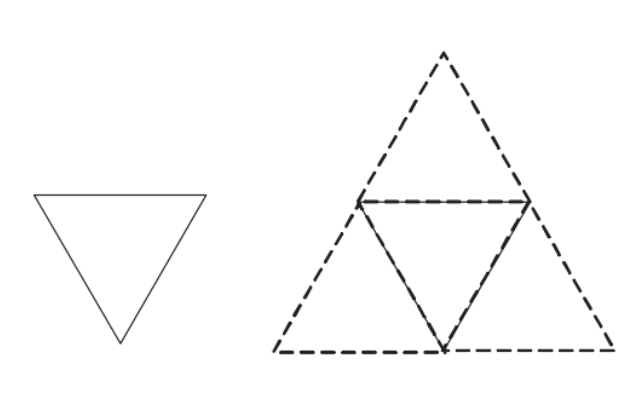
\includegraphics[scale=0.6]{img/triangles}
    \caption{Оптимальное расположение маячков}
    \label{optimum_placement}
\end{figure}

Расположение в узлах квадратов дает несколько худший результат (ошибка в среднем больше на 5,3\%), а случайное расположение маячков увеличивает ошибку на 34,9\% \cite{bulusu2001adaptive}.
